\documentclass[aspectratio=169]{beamer}
\usepackage[utf8]{inputenc}
%\usepackage[authordate,backend=biber,natbib]{biblatex-chicago}
%\usepackage{booktabs}
%\addbibresource{growthreferences.bib}

%\usepackage{utopia} %font utopia imported

\usetheme{Madrid}
\usecolortheme{beaver}

%------------------------------------------------------------
%This block of code defines the information to appear in the
%Title page
\title[Melitz (2003)] %optional
{The Impact of Trade on Intra-Industry Reallocations and Aggregate Industry Productivity}

\subtitle{Marc Melitz, \emph{Econometrica}, 2003}

\author [Hauk] % (optional)
{William~R.~Hauk,~Jr.} %\inst{1} %\and J.~Doe\inst{2}} 

\institute[UofSC] % (optional)
{
  %\inst{1}%
  Darla Moore School of Business\\
  University of South Carolina
  %\and
  %\inst{2}%
  %Faculty of Chemistry\\
  %Very Famous University
}

\date[ECON 860, Fall 2021] % (optional)
{ECON 860 -- International Trade Theory\\Fall 2021}

\logo{
\includegraphics[height=1cm]{UofSC_Monogram_Stack_CMYK_G.jpg}}

%End of title page configuration block

%---------------------------------------------------------

\AtBeginSection[]
{
  \begin{frame}
    \frametitle{Table of Contents}
    \tableofcontents[currentsection]
  \end{frame}
}

%------------------------------------------------------------

\begin{document}

%The next statement creates the title page.
\frame{\titlepage}

%-------------------------------------------------------------

\section{Introduction}

%-------------------------------------------------------------

\begin{frame}{Introduction}

\begin{itemize}
    \item<1-> Paper inspired by a spate of empirical literature showing that there is a large range of productivity differences among different establishments in the same industries.
    \item<2-> Stylized fact exists that more productive firms are more likely to export – even within ``export sectors” of an economy.
    \item<3-> Purpose of paper is to develop a dynamic model of an industry with heterogeneous firms to analyze the role of international trade in reallocating factors within an industry.
    \item<4-> Punchline is that model is consistent with observations that exposure to international trade.
\end{itemize}
    
\end{frame}

%--------------------------------------------------------------------

\begin{frame}{Existing Literature -- Empirical}

Empirical work supporting these stylized facts:

\begin{itemize}
    \item<1-> Bernard and Jensen (1999a); Aw, Chung, and Roberts (2000); Clerides, Lack, and Tybout (1998) all find that most productive firms self-select into export markets.
    \item<2-> Aw, Chung, and Roberts (2000); Pavcnik (2002) find that trade tends to reallocate resources from least productive firms to most productive firms.
    \item<3-> Bernard and Jensen (1999b) find that within-sector reallocations to more productive exporting plants account for 20\% of U.S. manufacturing productivity growth.
\end{itemize}
    
\end{frame}

%--------------------------------------------------------------------

\begin{frame}{Existing Literature -- Theory}

Model builds upon existing monopolistic competition and trade model of Krugman (1979).

\begin{itemize}
    \item<1-> Adds Hopenhayn’s (1992a, 1992b) model of heterogeneous firm selection in an industry – firms decide whether to enter a market when they are uncertain of their initial and future productivity.
    \item<2-> Adds insights from Bernard, Eaton, Jensen, and Kortum (2000) model of firm-specific comparative advantage.  But that paper holds the range of products produced exogenous.  This paper makes the range produced endogenous.
\end{itemize}
    
\end{frame}

%--------------------------------------------------------------------

\section{Setup of the Model}

\subsection{Demand}

%--------------------------------------------------------------------

\begin{frame}{Consumer Preferences}

\begin{itemize}
    \item<1-> Preferences of representative consumer are given by a C.E.S. utility function over a continuum of goods indexed by $ \omega $:
    \begin{equation*}
        U = \left[ \int_{\omega \in \Omega} {q\left( \omega \right)^{\rho} d\omega} \right]^{1/\rho}
    \end{equation*}
    where $ 0 < \rho < 1 $, which implies that the elasticity of substitution between any two goods is $ \sigma = \frac{1}{1 - \rho} > 1 $.
    \item<2-> Dixit and Stiglitz (1977) show that the set of varieties $ \Omega $  can be considered as an aggregate good $ Q = U $ associated with an aggregate price:
    \begin{equation*}
        P = \left[ \int_{\omega \in \Omega} {p\left( \omega \right)^{1 - \sigma} d\omega} \right]^{\frac{1}{1 - \sigma}}
    \end{equation*}
\end{itemize}
    
\end{frame}

%--------------------------------------------------------------------

\begin{frame}{Consumption and Expenditure Functions}

The optimal consumption and expenditure decisions for individual varieties is:
\begin{equation}
    \begin{split}
        q\left( \omega \right) &= Q\left[ \frac{p\left( \omega \right)}{P} \right]^{-\sigma} \\
        r\left( \omega \right) &= R\left[ \frac{p\left( \omega \right)}{P} \right]^{1 - \sigma}
    \end{split}
    \label{eq:quantityandexpenditure}
\end{equation}
where $ R = PQ = \int{\omega \in \Omega} r\left( \omega \right) d\omega $ represents aggregate expenditure.
    
\end{frame}

%--------------------------------------------------------------------

\subsection{Production}

%--------------------------------------------------------------------

\begin{frame}{Production Costs}

\begin{itemize}
    \item<1-> Each firm produces one variety $ \omega $ using one factor of production, labor, which is inelastically supplied at level $ L $.
    \item<2-> Labor is linearly related to the production of each variety using the function $ l = f + \frac{q}{\phi} $.  All firms have the same fixed cost $ f $, but they have different productivity levels indexed by $ \phi > 0 $. 
    \item<3-> With a C.E.S. utility function, the optimal markup over marginal cost is $ \frac{\sigma}{1 - \sigma} = \frac{1}{\rho} $, so the optimal price for variety $ \phi $ is:
    \begin{equation}
        p\left( \phi \right) = \frac{w}{\rho \phi}
        \label{eq:optimalprice}
    \end{equation}
\end{itemize}
    
\end{frame}

%--------------------------------------------------------------------

\begin{frame}{Firm Profit}

\begin{itemize}
    \item<1-> Firm profit is: CHECK THIS
    \begin{equation}
        \pi\left( \phi \right) = r\left( \phi \right) - l\left( \phi \right) = \frac{r\left( \phi \right)}{\sigma} - f
        \label{eq:profit1}
    \end{equation}
    where $ r\left( \phi \right) $ is firm revenue, which is a function of $ \phi $.
    \item<2-> Combining (\ref{eq:quantityandexpenditure}) and (\ref{eq:optimalprice}), we get:
    \begin{equation*}
        r\left( \phi \right) = R\left( P \rho \phi \right)^{\sigma - 1}
    \end{equation*}
    and plugging into (\ref{eq:profit1}), we get:
    \begin{equation*}
        \pi\left( \phi \right) = \frac{R}{\sigma}\left( P \rho \phi \right)^{\sigma - 1} - f
    \end{equation*}
\end{itemize}
    
\end{frame}

%--------------------------------------------------------------------

\begin{frame}{Comparing Firms}

\begin{itemize}
    \item<1-> If we compare any two firms’ outputs and revenues, we get:
    \begin{equation*}
        \frac{q\left( \phi_{1} \right)}{q\left( \phi_{2} \right)} = \left( \frac{\phi_{1}}{\phi_{2}} \right)^{\sigma}
    \end{equation*}
    and
    \begin{equation}
        \frac{r\left( \phi_{1} \right)}{r\left( \phi_{2} \right)} = \left( \frac{\phi_{1}}{\phi_{2}} \right)^{\sigma - 1}
        \label{eq:relativerevenue}
    \end{equation}
    \item<2-> So, a more productive firm will have higher output, higher revenues, and lower price, and earn higher profits than firms with lower productivity.
\end{itemize}
    
\end{frame}

%--------------------------------------------------------------------

\subsection{Equilibrium Characterization}

%--------------------------------------------------------------------

\begin{frame}{Equilibrium Characterization}

\begin{itemize}
    \item<1-> An equilibrium is characterized by a mass of firms $ M $ and a distribution of productivity levels $ \mu\left( \phi \right) $.  The aggregate price level $ P $ is then:
    \begin{equation*}
        P = \left[ \int_{0}^{\infty} p\left( \phi \right)^{1 - \sigma} M \mu\left( \phi \right) d\phi \right]^{\frac{1}{1 - \sigma}}
    \end{equation*}
    \item<2-> Using the pricing rule from (\ref{eq:optimalprice}), this can be written as:
    \begin{equation*}
        P = M^{\frac{1}{1 - \sigma}} p\left( \tilde{\phi} \right)
    \end{equation*}
    where:
    \begin{equation*}
        \tilde{\phi} = \left[ \int_{0}^{\infty} \phi^{\sigma - 1} \mu\left( \phi \right) d\phi \right]^{\frac{1}{\sigma - 1}}
    \end{equation*}
\end{itemize}
    
\end{frame}

%--------------------------------------------------------------------

\begin{frame}{Equilibrium Characterization}

\begin{itemize}
    \item<1-> It is shown in the Appendix that $ \tilde{\phi} $ is a sufficient statistic to summarize the distribution $ \mu\left( \phi \right)$.
    \item<2-> The aggregate variables can be derived as:
    \begin{equation*}
        \begin{split}
           P &= M^{\frac{1}{1 - \sigma}} p\left( \tilde{\phi} \right) \\
           R = PQ &= M r\left( \tilde{\phi} \right) \\
           Q &= M^{\frac{1}{\rho}} q\left( \tilde{\phi} \right) \\
           \Pi &= M \pi \left( \tilde{\phi} \right)
        \end{split}
    \end{equation*}
\end{itemize}
    
\end{frame}

%--------------------------------------------------------------------

\section{Firm Entry and Exit}

%--------------------------------------------------------------------

\begin{frame}{Productivity Draws}

\begin{itemize}
    \item<1-> Prior to entry, firms are identical.  To enter a market, firms must make a fixed investment $ f_{e} > 0 $, which is treated as a sunk cost once incurred.  Once firms enter the market, they received a productivity level $ \phi $ drawn from a common density function $ g\left( \phi \right) $, which has a cumulative distribution $ G\left( \phi \right) $.
    \item<2-> Once a firm knows its productivity level, it can decide to produce or not produce.  If it does produce, it will face a probability $ \delta $ in every period that it will suffer a shock that causes it to exit the market.
    \item<3-> If there is no time discounting, then each firm’s value function is:
    \begin{equation*}
        v\left( \phi \right) = \max\left\{ 0, \sum_{t = 1}^{\infty }{\left( 1 - \delta \right)^{t}} \pi\left( \phi \right)\right\} = \max\left\{ 0, \frac{1}{\delta} \pi\left( \phi \right) \right\}
    \end{equation*}
\end{itemize}
    
\end{frame}

%--------------------------------------------------------------------

\begin{frame}{Firm Exit and Productivity}

\begin{itemize}
    \item<1-> Define $ \phi^{*} $ as the lowest productivity level for firms that are producing.  Because $ \pi\left( 0 \right) = - f_{e} $, then $ \pi\left( \phi^{*} \right) = 0 $.
    \item<2-> Since subsequent firm exit is random, $ \mu\left( \phi \right) $ can be defined as the subset of $ g\left( \phi \right) $ that is above $ \phi^{*} $:
    \begin{equation*}
        \mu\left( \phi \right) = \left\{ \begin{matrix}
           \frac{g\left( \phi \right)}{1 - G\left( \phi^{*} \right)} \text{ if } \phi > \phi^{*} \\
           0 \text{ otherwise}
        \end{matrix} \right\}
    \end{equation*}
    \item<3-> So, aggregate productivity is the expected value of $ \phi $ conditional on being greater than $ \phi^{*} $:
    \begin{equation*}
        \tilde{\phi}\left( \phi^{*} \right) = \left[ \frac{1}{1 - G\left( \phi^{*} \right)} \int_{\phi^{*}}^{\infty } \phi^{\sigma - 1} g\left( \phi \right) d\phi \right]^{\frac{1}{\sigma - 1}}
    \end{equation*}
\end{itemize}
    
\end{frame}

%--------------------------------------------------------------------

\subsection{Zero Profit Cutoff Condition}

%--------------------------------------------------------------------

\begin{frame}{Zero Profit Cutoff Condition}

\begin{itemize}
    \item<1-> Since the average productivity level is determined by $ \phi^{*} $, the average revenue and profit levels are as well.  Using equation (\ref{eq:relativerevenue}), we can derive:
    \begin{equation*}
        \tilde{r} = r\left( \tilde{\phi} \right) = \left( \frac{\tilde{\phi}\left( \phi^{*} \right)}{\phi^{*}} \right)^{\sigma - 1} r\left( \phi^{*} \right)
    \end{equation*}
    \item<2-> Which, combined with (\ref{eq:profit1}), implies an average profit of:
    \begin{equation*}
        \tilde{\pi} = \pi\left( \tilde{\phi} \right) = \left( \frac{\tilde{\phi}\left( \phi^{*} \right)}{\phi^{*}} \right)^{\sigma - 1} \frac{r\left( \phi^{*} \right)}{\sigma} - f_{e}
    \end{equation*}
    \item<3-> Because we have a zero-profit condition at $ \pi\left( \phi^{*} \right) = 0 $, then we can combine the above equations to derive:
    \begin{equation}
        \pi\left( \phi^{*} \right) = 0 \Leftrightarrow r\left( \phi^{*} \right) = \sigma f_{e} \Leftrightarrow \tilde{\pi} = f_{e} k\left( \phi^{*} \right)
        \label{eq:zerocutoffcondition}
    \end{equation}
    where $ k\left( \phi^{*} \right) = \left( \frac{\tilde{\phi}\left( \phi^{*} \right)}{\phi^{*}} \right)^{\sigma - 1} - 1 $.
\end{itemize}
    
\end{frame}

%--------------------------------------------------------------------

\subsection{Free Entry and the Value of Firms}

%--------------------------------------------------------------------

\begin{frame}{Free Entry and the Value of Firms}

\begin{itemize}
    \item<1-> All incumbent firms, except for the zero-profit cutoff firm, earn positive profits – indeed, the expectation of earning profits is the reason that they invest in the fixed cost of entry $ f_{e} $.  Let $ \tilde{v} = \frac{\tilde{\pi}}{\delta} $ be the present discounted value of average profit flows conditional on successful entry.  We can derive the expected value of entry as:
    \begin{equation*}
        v_{e} = \frac{1 - G\left( \phi^{*} \right)}{\delta} \tilde{\pi} - f_{e}
    \end{equation*}
    \item<2-> In equilibrium, this value cannot be negative, or firms would not want to enter.  It also cannot be positive if there is free entry.  Therefore, the free entry condition implies that $ v_{e} = 0 $, or:
    \begin{equation}
        \tilde{\pi} = \frac{\delta}{1 - G\left( \phi^{*} \right)} f_{e}
        \label{eq:freeentrycondition}
    \end{equation}
\end{itemize}
    
\end{frame}

%--------------------------------------------------------------------

\section{Equilibrium in a Closed Economy}

%--------------------------------------------------------------------

\begin{frame}{Closed Economy Equilibrium}

\begin{itemize}
    \item<1-> Equations (\ref{eq:zerocutoffcondition}) and (\ref{eq:freeentrycondition}) give us two equations that depend on $ \tilde{\pi} $ and $ \phi^{*} $:
    \begin{equation*}
        \begin{split}
             \tilde{\pi} &= \left[ \left( \frac{\tilde{\phi}\left( \phi^{*} \right)}{\phi^{*}} \right)^{\sigma - 1} - 1 \right] f_{e} \\
             \tilde{\pi} &= \frac{\delta}{1 - G\left( \phi^{*} \right)} f_{e}
        \end{split}
    \end{equation*}
    \item<2-> For the first equation, $ \frac{\tilde{\phi}\left( \phi^{*} \right)}{\phi^{*}} $ goes from $ \infty $  to $ 1 $ (and $ \tilde{\pi} $ goes from $ \infty $  to $ 0 $) as $ \phi^{*} $ goes from $ 0 $ to $ \infty $.
    \item<3-> For the second equation, $ G\left( \phi^{*} \right) $ goes from $ 0 $ to $ 1 $ (and $ \tilde{\pi} $ goes from $ \delta f_{e} $ to $ \infty $) as $ \phi^{*} $ goes from $ 0 $ to $ \infty $. 
\end{itemize}
    
\end{frame}

%--------------------------------------------------------------------

\begin{frame}{Figure 1}

These two curves must cross once, and we get Figure 1:

\begin{figure}
    \centering
    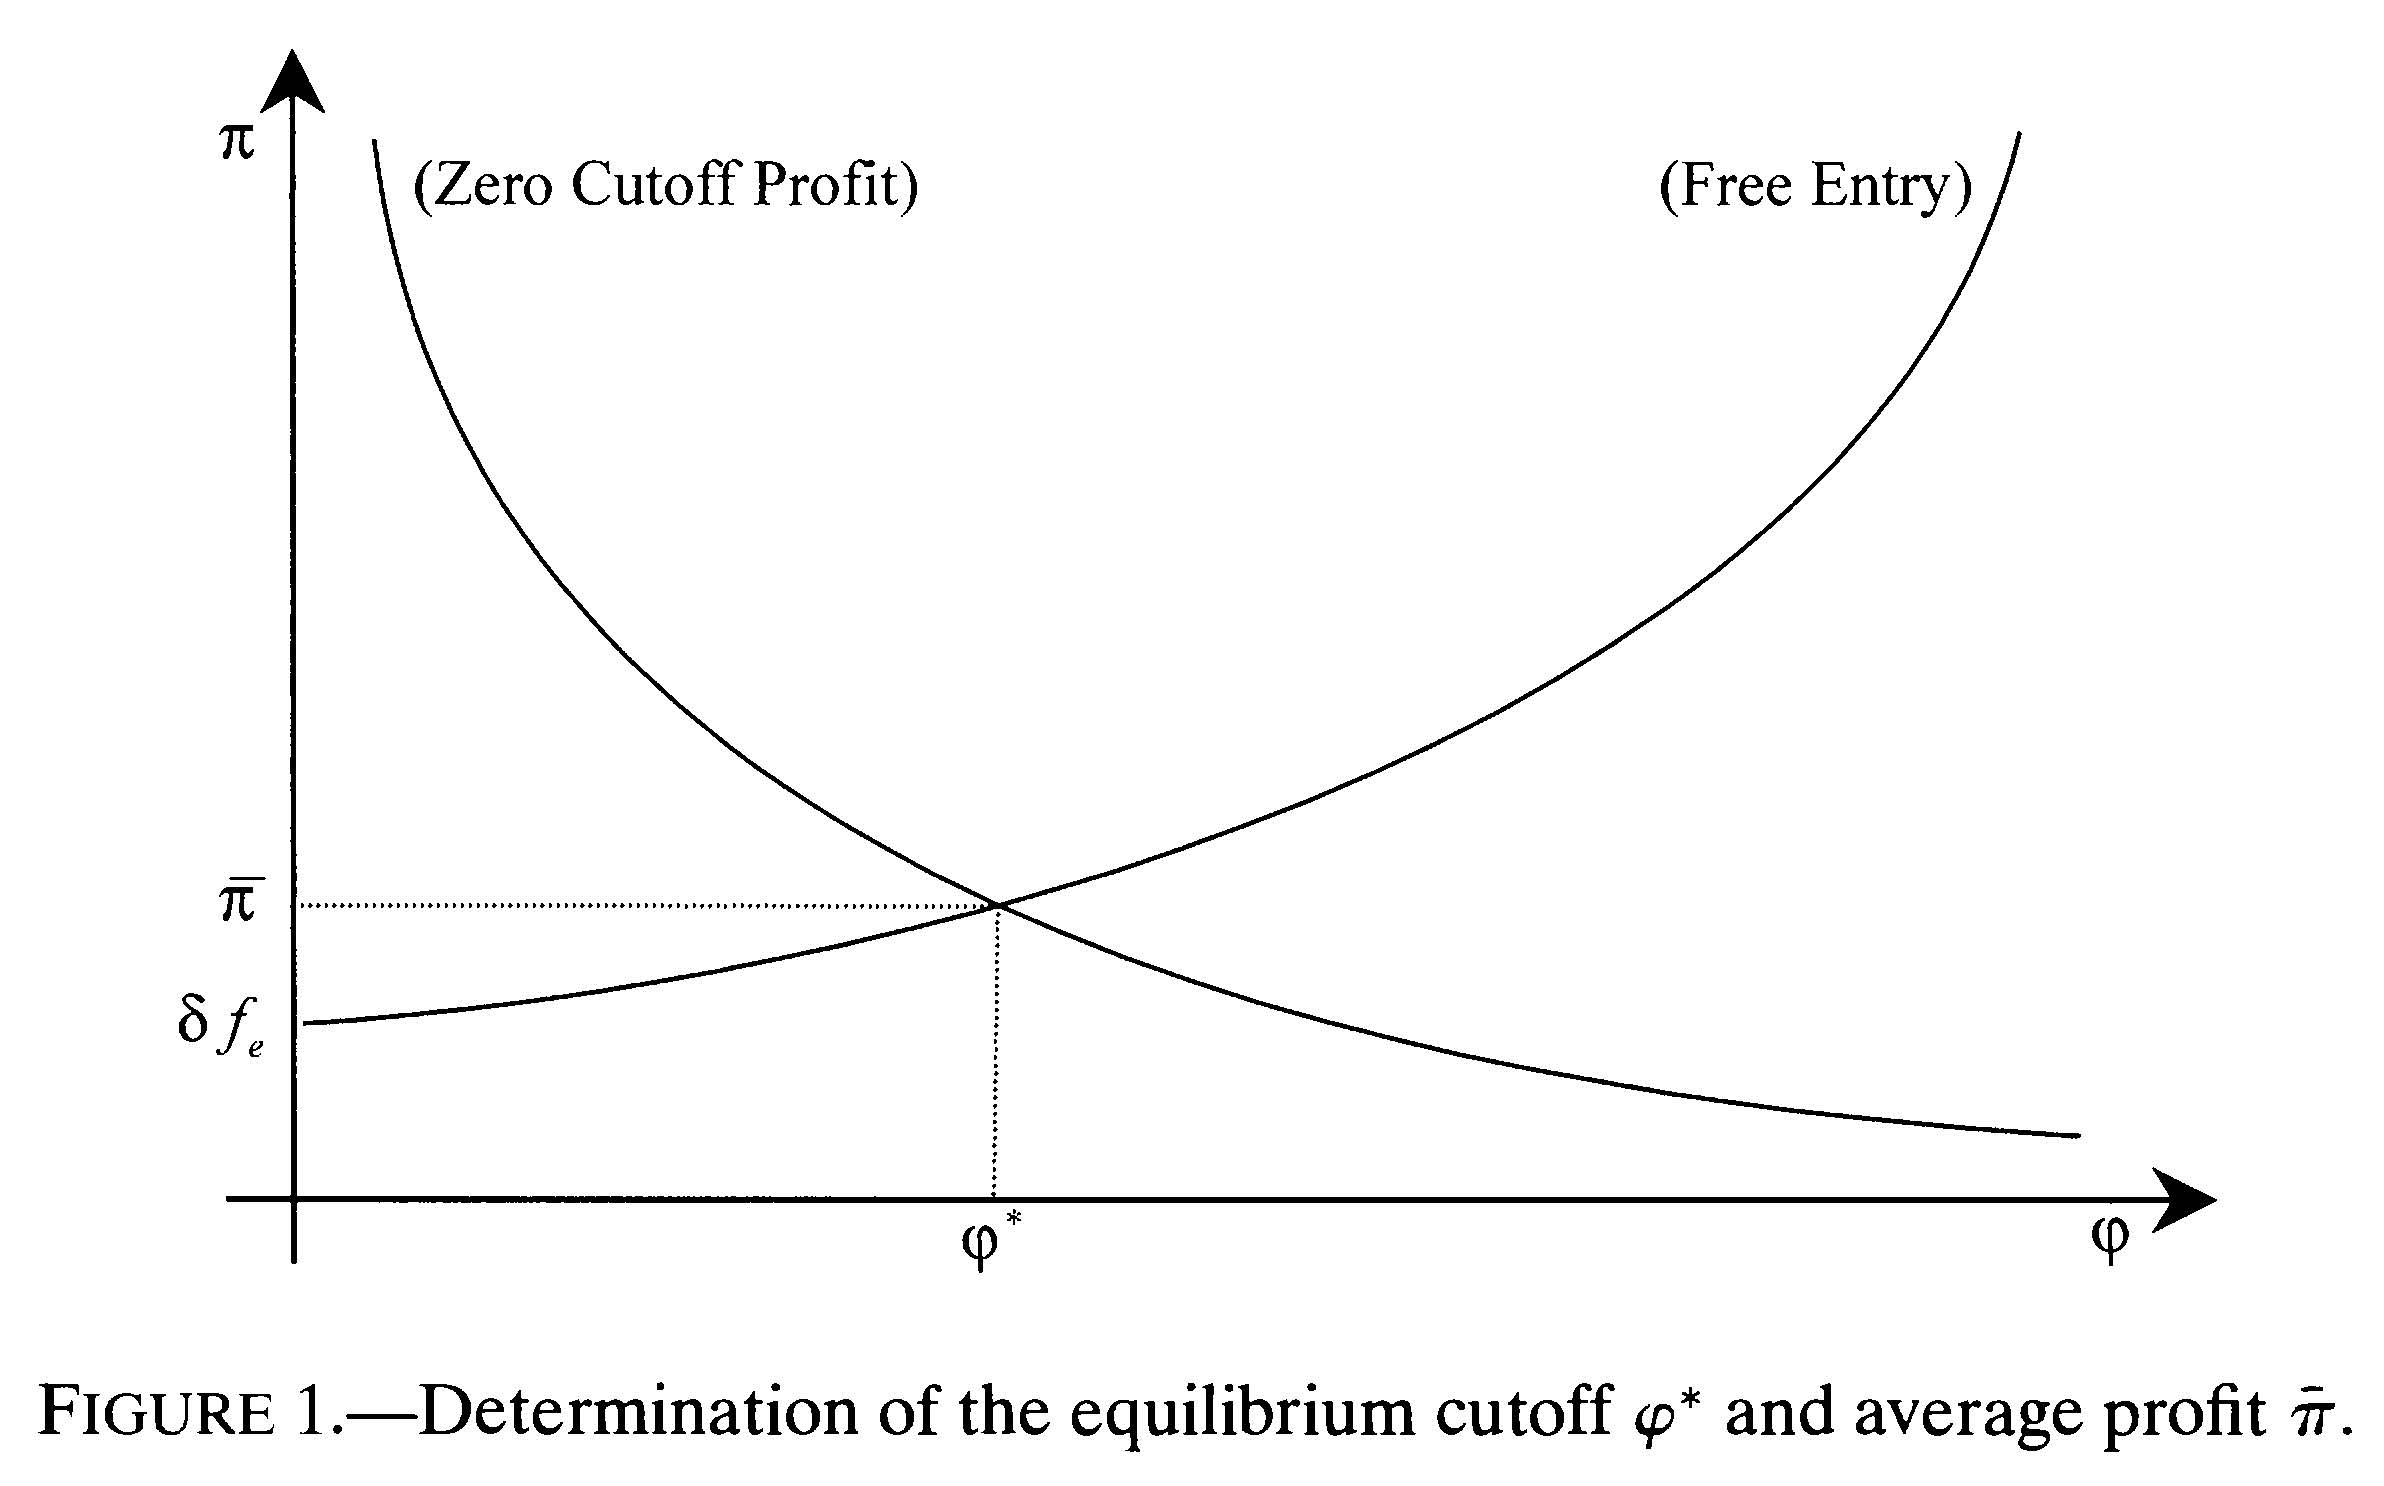
\includegraphics{MelitzFig1.jpg}
    \label{fig:Fig1}
\end{figure}
    
\end{frame}

%--------------------------------------------------------------------

\begin{frame}{Stationary Equilibrium}

\begin{itemize}
    \item<1-> To have a stationary equilibrium, the number of successful new entrants must equal the number of firms that are kicked out of the market $ p_{in} M_{e} = \delta M $.
    \item<2->  Some of our labor supply must be used for investment on the part of the firms entering the market, so labor market clearing requires that $ L = L_{p} + L_{e} $ where $ L_{p} $ is the number of workers in production, and $ L_{e} $ is the number of workers used in investment by firms entering.
    \item<3->  Payments to production workers must equal the difference between revenue and profits: $ L_{p} = R - \Pi $.
\end{itemize}
    
\end{frame}

%--------------------------------------------------------------------

\begin{frame}{Number of Firms in Equilibrium}

\begin{itemize}
    \item<1-> Using this market clearing condition and the free entry condition, $ L_{e} $ can be written as:
    \begin{equation*}
        L_{e} = M_{e} f_{e} = \frac{\delta M}{P_{in}} f_{e} = M \tilde{\pi} = \Pi
    \end{equation*}
    so aggregate revenue must equal total payments to labor.
    \item<2-> The mass of producing firms in any period can be determined from the average profit level:
    \begin{equation*}
        M = \frac{R}{\tilde{r}} = \frac{L}{\sigma\left( \tilde{\pi} + f_{e} \right)}
    \end{equation*}
    \item<3-> Knowing the mass of firms $ M $, in turn, pins down the equilibrium price index:
    \begin{equation*}
        P = M^{\frac{1}{1 - \sigma}} p\left( \phi \right) = \frac{M^{\frac{1}{1 - \sigma}}}{\rho \tilde{\phi}}
    \end{equation*}
\end{itemize}
    
\end{frame}

%--------------------------------------------------------------------

\begin{frame}{Analysis of the Equilibrium}

\begin{itemize}
    \item<1-> All of the firm-level variables are independent of the country size $ L $.  Welfare per worker is given by:
    \begin{equation*}
        W = P^{-1} = M^{\frac{1}{1 - \sigma}} \rho \tilde{\phi}
    \end{equation*}
    which increases in $ M $ solely due to increased product variety.  (This is the result from Krugman (1980).)
    \item<2->  While the results of this section are identical to a model where $ \phi $ is exogenously given for all firms, the heterogeneous nature of the firms will be important when the country is exposed to trade, which induces reallocations of labor across firms.  
\end{itemize}
    
\end{frame}

%--------------------------------------------------------------------

\section{Overview and Assumptions of the Open Economy Model}

%--------------------------------------------------------------------

\begin{frame}{Assumptions of the Open Economy Model}

\begin{itemize}
    \item<1->  In the absence of any costs to trade, the combined market can be represented as an integrated economy, with a greater variety of goods for consumers, like Krugman (1979, 1980).
    \item<2->  Melitz assumes (in line with evidence, Roberts and Tybout (1977)) that exporting firms face, not only marginal costs to trade, but also fixed costs.
    \item<3-> Firms make export decisions \emph{after} they know about their own productivity level (unlike original market entry decision).
    \item<4-> Per-unit trade costs (which could include tariffs or export taxes) are modeled in an “iceberg” fashion – $ \tau > 1 $ units of a good must be shipped in order for $ 1 $ to arrive.
    \item<5-> Countries are similar enough in size to generate factor price equalization, however, the world consists of $ n + 1 \ge 2 $ countries.  Each country that a firm decides to enter incurs a fixed investment cost of $ f_{ex} > 0 $.
\end{itemize}
    
\end{frame}

%--------------------------------------------------------------------

\section{Equilibrium in the Open Economy}

%--------------------------------------------------------------------

\begin{frame}{Equilibrium in the Open Economy \#1}

\begin{itemize}
    \item<1-> Symmetry assumption ensures that all countries have the same wage, which is still normalized to one, and they also have the same aggregate variables.
    \item<2-> Pricing for sales in the domestic market is the same as before:
    \begin{equation*}
        p_{d}\left( \phi \right) = \frac{w}{\rho \phi} = \frac{1}{\rho \phi}
    \end{equation*}
    but if we sell in a foreign market, we pay a transaction cost of $ \tau $, which makes the optimal price to charge in the foreign market:
    \begin{equation*}
        p_{x}\left( \phi \right) = \frac{\tau}{\rho \phi} = \tau p_{d}\left( \phi \right)
    \end{equation*}
    \item<3-> Revenues earned from domestic sales will then be $ r_{d}\left( \phi \right) = R\left( P \rho \phi \right)^{\sigma - 1} $ and for export sales $ r_{x}\left( \phi \right) = \tau^{1 - \sigma} r_{d}\left( \phi \right) $, where $ R $ and $ P $ represent aggregate expenditures and the price index in each country.
\end{itemize}
    
\end{frame}

%--------------------------------------------------------------------

\begin{frame}{Equilibrium in the Open Economy \#2}

\begin{itemize}
    \item<1-> The total revenue of a firm then becomes:
    \begin{equation*}
        r\left( \phi \right) = \left\{ \begin{matrix}
             r_{d}\left( \phi \right) \text{ if the firm does not export} \\
             r_{d}\left( \phi \right) + nr_{x}\left( \phi \right) = \left( 1 + n\tau^{1 - \sigma} \right) r_{d}\left( \phi \right) \text{ if the firm exports to all countries}
        \end{matrix} \right\}
    \end{equation*}
    \item<2->  If some firms do not export, there will not be the same variety of goods available to all consumers in each country (even though our symmetry assumption means that the level of variety of goods available will be the same in all countries).
\end{itemize}
    
\end{frame}

%--------------------------------------------------------------------

\subsection{Firm Entry, Exit, and Export Status}

%--------------------------------------------------------------------

\begin{frame}{Firm Entry}

\begin{itemize}
    \item<1-> Firms face the same productivity distribution $ g\left( \phi \right) $ and a negative shock probability $ \delta $ that they did before trade.  As export costs and benefits are equal across countries, firms will either export everywhere or not export.
    \item<2-> Because there is no time discounting or export market uncertainty, firms are indifferent between paying $ f_{ex} $ as a one-time cost of $ f_{x} = \delta f_{ex} $ each period.  For notational simplicity, the paper uses the latter.
    \item<3-> Because a firm will never export and not also produce for the domestic market, we can represent the fixed overhead cost as a cost to the firm’s domestic profits:
    \begin{equation*}
        \begin{split}
            \pi_{d}\left( \phi \right) &= \frac{r_{d}\left( \phi \right)}{\sigma} - f \\
            \pi_{x}\left( \phi \right) &= \frac{r_{x}\left( \phi \right)}{\sigma} - f_{x}
        \end{split}
    \end{equation*}
\end{itemize}
    
\end{frame}

%--------------------------------------------------------------------

\begin{frame}{Firm Exporting Cutoff}

\begin{itemize}
    \item<1-> A firm that produces has a combined profit of:
    \begin{equation*}
        \pi\left( \phi \right) = \pi_{d}\left( \phi \right) + \max\left\{ 0, n\pi_{x}\left( \phi \right) \right\}
    \end{equation*}
    \item<2-> Firm value is given by:
    \begin{equation*}
        v\left( \phi \right) = \max \left\{ 0, \frac{\pi\left( \phi \right)}{\delta} \right\}
    \end{equation*}
    \item<3-> Similarly to the closed economy case, we can identify $ \phi^{*} = \inf \left\{ \phi : v\left( \phi \right) > 0 \right\} $, but we can also identify $ \phi_{x}^{*} = \inf \left\{ \phi : \phi \ge \phi^{*} \text{ and } \pi_{x}\left( \phi \right) > 0 \right\} $.
    \item<4-> If $ \phi_{x}^{*} > \phi^{*} $, then there are some firms that produce exclusively for the domestic market.  By definition, $ \pi_{d}\left( \phi^{*} \right) = 0 $ and $ \pi_{x}\left( \phi_{x}^{*} \right) = 0 $.
\end{itemize}
    
\end{frame}

%--------------------------------------------------------------------

\begin{frame}{Firm Partitioning}

\begin{itemize}
    \item<1-> This partitioning of firms will occur if $ \tau^{\sigma - 1} f_{x} > f $ -- in words, if the trade costs are relatively high compared to overhead production costs.
    \item<2-> If there are no fixed trade costs ($ f_{x} = 0 $), then no variable trade cost $ \tau $ will induce this partitioning.
    \item<3-> Conversely, a large enough fixed trade cost $ f_{x} > f $ will induce partitioning even in the absence of variable costs ($ \tau = 1 $).
    \item<4-> The probability of successful entry is $ p_{in} = 1 - G\left( \phi^{*} \right) $ and the probability of exporting for a successfully entering firm is: $ p_{x} = \frac{1 - G\left( \phi_{x}^{*} \right)}{1 - G\left( \phi^{*} \right)} $.
    \item<5-> Let $ M $ be the mass of firms in any country, $ M_{x} = p_{x}M $ be the number of exporting firms in any country, and $ M_{t} = M + nM_{x} $ be the number of varieties available to consumers in any country.
\end{itemize}
    
\end{frame}

%--------------------------------------------------------------------

\subsection{Aggregation}

%--------------------------------------------------------------------

\begin{frame}{Average Productivity Levels}

{\small
\begin{itemize}
    \item<1-> Let $ \tilde{\phi} = \tilde{\phi}\left( \phi^{*} \right) $ and $ \tilde{\phi}_{x} = \tilde{\phi}\left( \phi_{x}^{*} \right) $ be the average productivity levels for producing firms and exporting firms, respectively.
    \item<2-> Let $ \tilde{\phi}_{t} $ be the average productivity levels of the firms whose goods consumers are consuming:
    \begin{equation*}
        \tilde{\phi}_{t} = \left\{ \frac{1}{M_{t}} \left[ M \tilde{\phi}^{\sigma - 1} + nM_{x}\left( \frac{\tilde{\phi}_{x}}{\tau} \right)^{\sigma - 1} \right] \right\}^{\frac{1}{\sigma - 1}}
    \end{equation*}
    \item<3-> $ \tilde{\phi}_{t} $ is a useful statistic, because, similar to the closed economy equilibrium, it allows us to derive several variables of interest:
    \begin{equation*}
        \begin{split}
            P &= M_{t}^{\frac{1}{1 - \sigma}} p\left( \tilde{\phi}_{t} \right) = M_{t}^{\frac{1}{1 - \sigma}} \frac{1}{\rho \tilde{\phi}} \\
            R &= M_{t} r\left( \tilde{\phi} \right) \\
            W &= \frac{R}{L} M_{t}^{\frac{1}{1 - \sigma}} \rho \tilde{\phi}_{t}
        \end{split}
    \end{equation*}
\end{itemize}
}
    
\end{frame}

%--------------------------------------------------------------------

\begin{frame}{Average Revenue and Profit}

The average revenue $ \tilde{r} $ and profit $ \tilde{\pi} $ earned across all firms can be expressed as:
\begin{equation*}
    \begin{split}
        \tilde{r} &= r_{d}\left( \tilde{\phi} \right) + p_{x} n r_{x}\left( \tilde{\phi}_{x} \right) \\
        \tilde{\pi} &= \pi_{d}\left( \tilde{\pi} \right) + p_{x} n \pi_{x}\left( \tilde{\pi}_{x} \right)
    \end{split}
\end{equation*}
    
\end{frame}

%--------------------------------------------------------------------

\subsection{Equilibrium Conditions}

%--------------------------------------------------------------------

\begin{frame}{Average Profits}

\begin{itemize}
    \item<1-> Once again, using the relative revenue and profit conditions from equation (\ref{eq:relativerevenue}) we can derive:
    \begin{equation*}
        \begin{split}
            \pi_{d}\left( \phi^{*} \right) = 0 &\Leftrightarrow \pi_{d}\left( \tilde{\phi} \right) = f k\left( \phi^{*} \right) \\
            \pi_{x}\left( \phi_{x}^{*} \right) = 0 &\Leftrightarrow \pi_{x}\left( \tilde{\phi}_{x} \right) = f_{x} k\left( \phi_{x}^{*} \right)
        \end{split}
    \end{equation*}
    where $ k\left( \phi \right) = \left[ \frac{\phi^{*}\left( \phi \right)}{\phi} \right]^{\sigma - 1} - 1 $.
    \item<2-> We can also use (\ref{eq:relativerevenue}) to derive $ \phi_{x}^{*} $:
    \begin{equation*}
        \frac{r_{x}\left( \phi_{x}^{*} \right)}{r_{d}\left( \phi^{*} \right)} = \tau^{1 - \sigma} \left( \frac{\phi_{x}^{*}}{\phi^{*}} \right)^{\sigma - 1} = \frac{f_{x}}{f} \Leftrightarrow \phi_{x}^{*} = \phi^{*} \tau\left( \frac{f_{x}}{f} \right)^{\frac{1}{\sigma - 1}}
    \end{equation*}
\end{itemize}
    
\end{frame}

%--------------------------------------------------------------------

\begin{frame}{Cutoff Points}

\begin{itemize}
    \item<1-> We can then define the average profit $ \overline{\pi} $ as a function of the cutoff point $ \phi^{*} $:
    \begin{equation}
        \begin{split}
            \overline{\pi} &= \pi_{d}\left( \phi^{*} \right) + p_{x} n \pi_{x}\left( \tilde{\phi}_{x}^{*} \right) \\
            &= f k\left( \phi^{*} \right) + p_{x} n f_{x} k\left( \tilde{\phi}_{x}^{*} \right)
        \end{split}
        \label{eq:ZCPopen}
    \end{equation}
    this is the open-economy analog of the zero-profit cutoff (ZCP) condition.
    \item<2-> The firm valuation function, and therefore, the free-entry condition have not changed from the closed-economy version:
    \begin{equation*}
        v_{e} = 0 \Leftrightarrow \overline{\pi} = \frac{\delta f_{e}}{p_{in}}
    \end{equation*}
\end{itemize}
    
\end{frame}

%--------------------------------------------------------------------

\subsection{Determination of the Equilibrium}

%--------------------------------------------------------------------

\begin{frame}{Determining Equilibrium \#1}

\begin{itemize}
    \item<1-> The free-entry condition and the ZCP condition can be used to pin down an equilibrium $ \phi^{*} $ and $ \overline{\pi} $.
    \item<2-> The equilibrium $ \phi^{*} $ can be used, in turn, to derive $ \phi_{x}^{*} $, $ \tilde{\phi} $, $ \tilde{\phi}_{x} $, $ \tilde{\phi}_{t} $, and the ex-ante successful entry and export probabilities $ p_{in} $ and $ p_{x} $.
    \item<3-> In a stationary equilibrium, the mass of firms successfully entering is again equal to the mass of the firms exiting, $ p_{in} M_{e} = \delta M $, which means that the aggregate payment to investment workers $ L_{e} $ equals the profit level $ \Pi $.  Aggregate revenue is thus determined exogenously by the size of the labor force, $ R = L $. 
\end{itemize}

\end{frame}

%--------------------------------------------------------------------

\begin{frame}{Determining Equilibrium \#2}

\begin{itemize}
    \item<1-> Average firm revenue is determined by the ZCP and FE conditions:
    \begin{equation*}
        \overline{r} = r_{d}\left( \phi \right) + p_{x} n r_{x}\left( \tilde{\phi}_{x} \right) = \sigma \left( \overline{\pi} + f + p_{x} n f_{x} \right)
    \end{equation*}
    which, in turn, pins down the equilibrium mass of incumbent firms:
    \begin{equation}
        M = \frac{R}{\overline{r}} = \frac{L}{\sigma \left( \overline{\pi} + f + p_{x} n f_{x} \right)}
        \label{eq:firmswithtrade}
    \end{equation}
    \item<2-> Knowing the mass of firms in each country tells us the variety available in each country $ M_{t} = \left( 1 +n p_{x} \right) M $ and the price index $ P = M_{t}^{\frac{1}{1 - \sigma}} / \rho \tilde{\phi}_{t} $, which is the inverse of which is the real wage. 
\end{itemize}
    
\end{frame}

%--------------------------------------------------------------------

\section{The Impact of Trade}

%--------------------------------------------------------------------

\begin{frame}{Comparative Statics}

\begin{itemize}
    \item<1-> If we compare the ZCP for the closed economy:
    \begin{equation*}
        \overline{\pi} = f_{e} k\left( \phi^{*} \right)
    \end{equation*}
    and the ZCP for the open economy:
    \begin{equation*}
        \overline{\pi} = f_{e} k\left( \phi^{*} \right) + p_{x} n f_{x}\left( \phi_{x}^{*} \right)
    \end{equation*}
    it is clear that the opportunity to export shifts the ZCP curve upwards.
    \item<2-> Going back to Figure 1, this change would induce a higher cutoff productivity level: $ \phi^{*} > \phi_{a}^{*} $, and a higher average productivity level for each firm.
    \item<3-> Therefore, firms with productivity levels between $ \phi_{a}^{*} $ and $ \phi^{*} $ would exit the market when the country opened to trade (and the remaining firms would be more productive).
\end{itemize}
    
\end{frame}

%--------------------------------------------------------------------

\begin{frame}{Firm Numbers}

\begin{itemize}
    \item<1-> Looking at the number of firms in equation (\ref{eq:firmswithtrade}), it is clear that the number of firms will fall with trade.  Under reasonable parameter assumptions, it is probably the case that:
    \begin{equation*}
        M_{t} = \left( 1 + n p_{x} \right) M > M_{a}
    \end{equation*}
    although, if trade costs are high (and $ p_{x} $ is low) this may not be guaranteed.
    \item<2-> In the appendix, it is shown that, even if firm variety falls, the productivity gain in $ \overline{\pi} $ will always be large enough to guarantee a welfare gain. 
\end{itemize}
    
\end{frame}

%--------------------------------------------------------------------

\section{The Impact of Trade Liberalization}

%--------------------------------------------------------------------

\begin{frame}{The Impact of Trade Liberalization}

\begin{itemize}
    \item<1-> The previous section looked at an economy going from autarky to trade.
    \item<2-> This section looks at liberalization of trade as operationalized by changes in $ n $, $ \tau $, and $ f_{x} $.
    \item<3-> Increases in exposure to trade through any of these mechanisms will have similar results as moving from trade to autarky. 
\end{itemize}
    
\end{frame}

%--------------------------------------------------------------------

\begin{frame}{Increase in the Number of Trading Partners}

\begin{itemize}
    \item<1-> Looking at equation (\ref{eq:ZCPopen}), it is clear that an increase in $ n $ shifts the ZCP curve upwards.
    \item<2-> An upwards shift in ZCP increases the productivity cutoff level: $ \phi^{*'} > \phi^{*} $, as well as $ \phi_{x}^{*'} > \phi_{x}^{*} $.
    \item<3-> As a result, the least productive firms exit the market.  Some exporting firms will actually cease exporting, but the firms that do export will have higher profits.
    \item<4-> Market shares and profits are reallocated to the more efficient firms.
\end{itemize}
    
\end{frame}

%--------------------------------------------------------------------

\begin{frame}{Decrease in Variable Trade Costs}

\begin{itemize}
    \item<1-> A decrease in the variable trade cost $ \tau $ will have almost identical effects as the increase in trade partners.
    \item<2-> Decrease in $ \tau $ will cause the ZCP curve to shift upwards again, increasing the entry cutoff level $ \phi^{*} $.
    \item<3-> The big difference is that the export cutoff level $ \phi_{x}^{*} $ will fall.  So, the least productive firms will exit, but some middle level productivity firms will now export.
\end{itemize}
    
\end{frame}

%--------------------------------------------------------------------

\begin{frame}{Decrease in Fixed Trade Costs}

\begin{itemize}
    \item<1-> A decrease in the fixed export cost $ f_{x} $ will have a similar effect.
    \item<2-> Decrease in $ f_{x} $ will cause the ZCP curve to shift upwards again, increasing the entry cutoff level $ \phi^{*} $.
    \item<3-> The export cutoff level $ \phi_{x}^{*} $ will fall again.  So, the least productive firms will exit, but some middle level productivity firms will now export.
    \item<4-> The difference from a change in $ \tau $ is that only new exporting firms will see higher sales and profits.  Existing exporters will not see a change.
\end{itemize}
    
\end{frame}

%--------------------------------------------------------------------

\end{document}